\documentclass[zavrsnirad]{fer}
% Dodaj opciju upload za generiranje konačne verzije koja se učitava na FERWeb
% Add the option upload to generate the final version which is uploaded to FERWeb

\usepackage{float}
\usepackage{blindtext}
\usepackage{xcolor}
\usepackage{listings}

\lstset{ %
	language=Python,
	basicstyle=\ttfamily\footnotesize,
	keywordstyle=\color{blue},
	commentstyle=\color{green},
	stringstyle=\color{red},
	showstringspaces=false,
	frame=single,
	numbers=left,
	numberstyle=\tiny\color{gray},
	breaklines=true,
	breakatwhitespace=true,
	tabsize=2
}

\usepackage[labelfont=bf]{caption}

\usepackage{changepage} % For adjusting margins
\usepackage{multirow}
\usepackage{multicol}

% \usepackage[section]{placeins} % To prevent figures from going into the next section
\usepackage{placeins} % For FloatBarrier

% Define a thicker table line
\usepackage{array}

\makeatletter
\newcommand{\thickhline}{%
	\noalign {\ifnum 0=`}\fi \hrule height 1pt
	\futurelet \reserved@a \@xhline
}

\usepackage{enumitem}
\setlist[itemize]{noitemsep}

\usepackage[justification=centering]{caption}

\usepackage{fixltx2e}

%--- PODACI O RADU / THESIS INFORMATION ----------------------------------------

% Naslov na engleskom jeziku / Title in English
\title{Optical character recognition system for older books in Croatian}

% Naslov na hrvatskom jeziku / Title in Croatian
\naslov{SUSTAV ZA OPTIČKO RASPOZNAVANJE TEKSTA STARIJIH KNJIGA NA HRVATSKOME JEZIKU}

% Broj rada / Thesis number
\brojrada{1605}

% Autor / Author
\author{Dominik Agejev}

% Mentor 
\mentor{Prof.\@ Tomislav Hrkać}

% Datum rada na engleskom jeziku / Date in English
\date{September, 2024}

% Datum rada na hrvatskom jeziku / Date in Croatian
\datum{rujan, 2024.}

%-------------------------------------------------------------------------------


\begin{document}


% Naslovnica se automatski generira / Titlepage is automatically generated
\maketitle


%--- ZADATAK / THESIS ASSIGNMENT -----------------------------------------------

% Zadatak se ubacuje iz vanjske datoteke / Thesis assignment is included from external file
% Upiši ime PDF datoteke preuzete s FERWeb-a / Enter the filename of the PDF downloaded from FERWeb
\zadatak{hr_0036537505_73.pdf}


%--- ZAHVALE / ACKNOWLEDGMENT --------------------------------------------------

\begin{zahvale}
  % Ovdje upišite zahvale / Write in the acknowledgment
  Jakovu, Lovri i Roku,
  hvala na pomoći!
\end{zahvale}


% Odovud započinje numeriranje stranica / Page numbering starts from here
\mainmatter


% Sadržaj se automatski generira / Table of contents is automatically generated
\tableofcontents


%--- UVOD / INTRODUCTION -------------------------------------------------------
\chapter{Uvod}
\label{pog:uvod}

Cilj rada nadići je uspješnost gotovih sustava za optičko raspoznavanje teksta (eng. \textit{Optical Character Recognition} ili \textit{OCR}) na starijim knjigama hrvatskoga jezika koristeći se nenadziranim metodama učenja, odnosno bez označenih podataka za trening modela, uz predobradu i naknadnu obradu.

Iako suvremeni sustavi poput DTrOCR-a \cite{Fujitake2023} postižu gotovo savršene rezultate u raznim primjenama, optičko raspoznavanje teksta  nipošto nije riješen problem. Još uvijek i najbolji sustavi, poput gore navedenog, pogrešno prepoznaju više od 10\% riječi na fotografijama teksta „u divljini“ i gotovo 20\% riječi u rukopisima na kineskom jeziku.

Uz to, zbog ovisnosti o jezičnim modelima, novija rješenja općenito nisu primjenjiva bez dodatne prilagodbe na manje zastupljene jezike, poput hrvatskog, ili se pak oslanjaju na veliku količinu označenih podataka ili na sintetičke podatke, generirane modelima koji za rjeđe jezike nisu dostupni, te zahtijevaju značajne računalne resurse.

Nadalje, zbog suviše uske primjene, specifični problemi, poput predmeta ovog rada, raspoznavanja teksta antikvarnih knjiga i to na jeziku ograničene uporabe, redovito se zaobilaze u prilog doprinosima aktualnim primjenama. \cite{Olejniczak2022}

U okviru ovog rada najprije se uvodi u područje, metode i temeljne pojmove koji će se koristiti u radu. Zatim je detaljno izložen zadatak i njegove specifičnosti uz pregled dosadašnjih postignuća unutar područja.

Prelazeći na izvedbu rješenja, razmatraju se najznačajniji slobodno dostupni OCR alati prikladni zadatku, a to su Tesseract \cite{Smith2007}, OCR sustav opće namjene koji održava Google, te Ocular \cite{Berg2013}, razvijen specifično za primjenu na antikvarnim dokumentima.

Nakon treniranja i optimiziranja hiperparametara Oculara, uspoređen je s Tesseractom na već predobrađenim ispitnim podacima gdje se pokazuje da usprkos starijoj arhitekturi u bitnome nadjačava Tesseract, ali uz određena ograničenja.

Konačno, izveden je sustav glasanja kojim se postiže veća uspješnost od one samostalnih modela.


%	\begin{figure}[htb]
%	  \centering
%	  \includegraphics[width=0.38\linewidth]{Figures/lenovo_yoga_tab3_pro_front.png} 
%	  \caption{Moja prva slika}
%	  \label{slk:prvaslika}
%	\end{figure}

% Referenciramo se na sliku \ref{slk:prvaslika} u sredini rečenice, zatim prije zareza \ref{slk:prvaslika}, te zatim na kraju rečenice \ref{slk:prvaslika}.
% Upravo smo testirali radi li naredba \verb|\ref| ispravno u slučaju kada nakon nje slijedi točka.


%-------------------------------------------------------------------------------
\chapter{Uvod u OCR}
\label{pog:ocr_uvod}

Optičko raspoznavanje teksta grana je računalnog vida koja se bavi izdvajanjem teksta iz slika, bilo dokumenata, rukopisa ili scenskih fotografija, radi lakog pretraživanja i uređivanja, jednostavnijeg arhiviranja ili pak dostupnosti sadržaja slabovidnima i slijepima.

U odnosu na sadržaj ulaznih slika najčešće govorimo o prepoznavanju teksta tiskanih dokumenata, rukopisa ili teksta „u divljini“, npr. natpisa na pročeljima trgovina, s tim da je potonje uže povezano s drugim granama računalnog vida poput detekcije i klasifikacije objekata.

OCR sustavi često se razvijaju i za još uže definirane zadatke, primjerice prepoznavanje teksta na računima ili antikvarnim dokumentima. Takvi sustavi, kakvima se bavi i ovaj rad, nazivaju se jednonamjenskima (eng. \textit{task-specific}), dok se sustavi prilagođeni raznim uporabama zovu sustavima opće namjene (eng. \textit{general purpose}). \cite{Borovikov2014}

Optičko raspoznavanje teksta podrazumijeva u bitnome pet koraka: predobradu, segmentaciju, izdvajanje značajki, klasifikaciju te naknadnu obradu. \cite{Dhande2017} U ovom poglavlju izložit će se ugrubo najznačajnije metode i pojmovi koji će se koristiti u ostatku rada.

\section{Predobrada}

Predobrada se odnosi na postupak prilagodbe ulazne slike radi uspješnijeg raspoznavanja znakova. Načela po kojima se ravna predobrada uključuju pojednostavljenje ulaza izostavljanjem nebitnih informacija, što čine binarizacija i eliminacija šuma, te ispravljanje fizičkih nesavršenosti, uzrokovanih bilo tiskom bilo digitalizacijom ulaza, što rade metode poput ispravljanja nagnuća (eng. \textit{skew correction}).

\subsection{Binarizacija}
\label{Binarizacija}

Cilj binarizacije razlučivanje je između teksta i pozadine. Najjednostavniji način za to postavljanje je praga (eng. \textit{thresholding}) za koji su svi pikseli s RGB ili sivotonskim (eng. \textit{grayscale}) vrijednostima nižim od praga obojani crno, tj. označeni kao tekst, a pikseli iznad praga označeni kao pozadina. \cite{Jyotsna2016}

\begin{figure}[hbt]
	\centering
	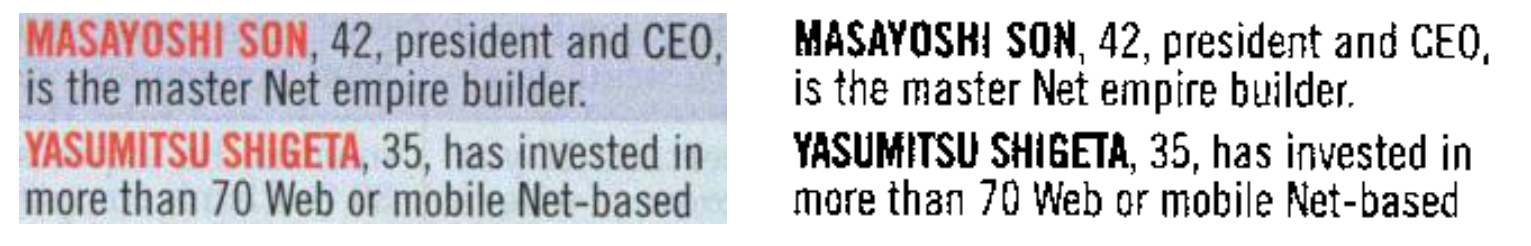
\includegraphics[width=0.9\linewidth]{Figures/binarization.png} 
	\caption{Primjer binarizacije \cite{binarization-image}}
	\label{slk:binarizacija}
\end{figure}

Razlikujemo globalne i lokalne metode binarizacije. Globalne, poput često korištene Otsuove  metode \cite{Otsu1979}, postavljaju jedan prag za cijeli dokument, što je vremenski učinkovito i uspješno u idealnom slučaju s jednoličnom pozadinom, no zakazuje pri nejednakom osvjetljenju ili sjeni uslijed loše skeniranog pregiba knjige. Lokalne, poput metode adaptivnog kontrasta \cite{Su2013}, temeljenoj na prepoznavanju rubova pomoću kontrasta susjednih piksela, nešto su resursno zahtjevnije, ali zato daju bolje rezultate. \cite{Otsu1979, Su2013}

\subsection{Ispravljanje nagnuća}

Cilj ispravljanja nagnuća zaokrenuti je retke teksta tako da su vodoravni. Utvrđivanje kuta nagnuća redaka binarizirane slike može se svesti na pronalazak pravca koji najbolje aproksimira redak, a u tu svrhu najčešće se koristi Houghova transformacija. \cite{Hassanein2015} Konceptualno, Houghova transformacija za svaku rubnu točku slike pronalazi parametre (m, c) pravaca koji se kroz nju mogu provući. Pronađeni skup parametara zapravo je pravac u m, c prostoru, a odredivši pripadajući pravac svakoj točci, ako neki pravci imaju zajedničko sjecište, kroz njima pripadne točke moguće je povući pravac koji u konkretnom slučaju određuje redak teksta.

\section{Segmentacija}

Segmentacija podrazumijeva razlučivanje semantički značajne dijelove slike od kojih su najbitniji retci, riječi i znakovi te koji se obično tim redom i pronalaze: retci u slici, riječi u retku, znakovi u riječi.

Najjednostavnija metoda segmentacije gradi histogram piksela teksta te postavlja granice između elemenata gdje ima najviše piksela pozadine.

\begin{figure}[hbt]
	\centering
	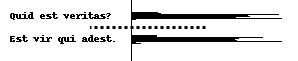
\includegraphics[width=0.9\linewidth]{Figures/line-segmentation.png} 
	\caption{Linijska segmentacija histogramom}
	\label{slk:histogram}
\end{figure}

\section{Izdvajanje značajki}

Starije metode OCR-a, prije prelaska na neuronske mreže, koristile su ručno definirane značajke, poput tzv. Granlundovih opisnika temeljenih na Fourierovoj transformaciji \cite{Trier1996} ili jednostavnih matrica koje predstavljaju oblik znaka, kao na slici \ref{slk:jednostavna-matrica},  dok u suvremenim sustavima poput Tesseracta raniji slojevi neuronske mreže izdvajaju značajke, a kasniji provode klasifikaciju teksta.

\begin{figure}[hbt]
	\centering
	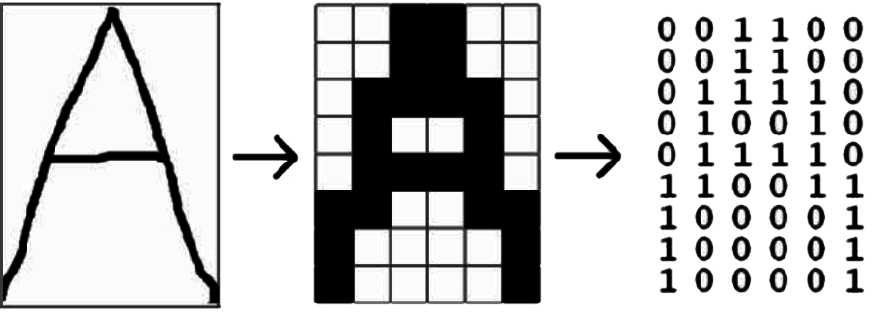
\includegraphics[width=0.7\linewidth]{Figures/simple-letter-matrix.png}
	\caption{Tvorba predloška znaka \cite{Noaman2015}}
	\label{slk:jednostavna-matrica}
\end{figure}

Za izdvajanje značajki koriste se konvolucijske neuronske mreže (CNN) koje se mogu predočiti kao niz filtera, od kojih prvi provjeravaju npr. je li određeni rub ili ugao prisutan u znaku, a kasniji slojevi zadržavajući najbitnije informacije uče općenitija pravila. \cite{IBM}

\begin{figure}[h!]
	\centering
	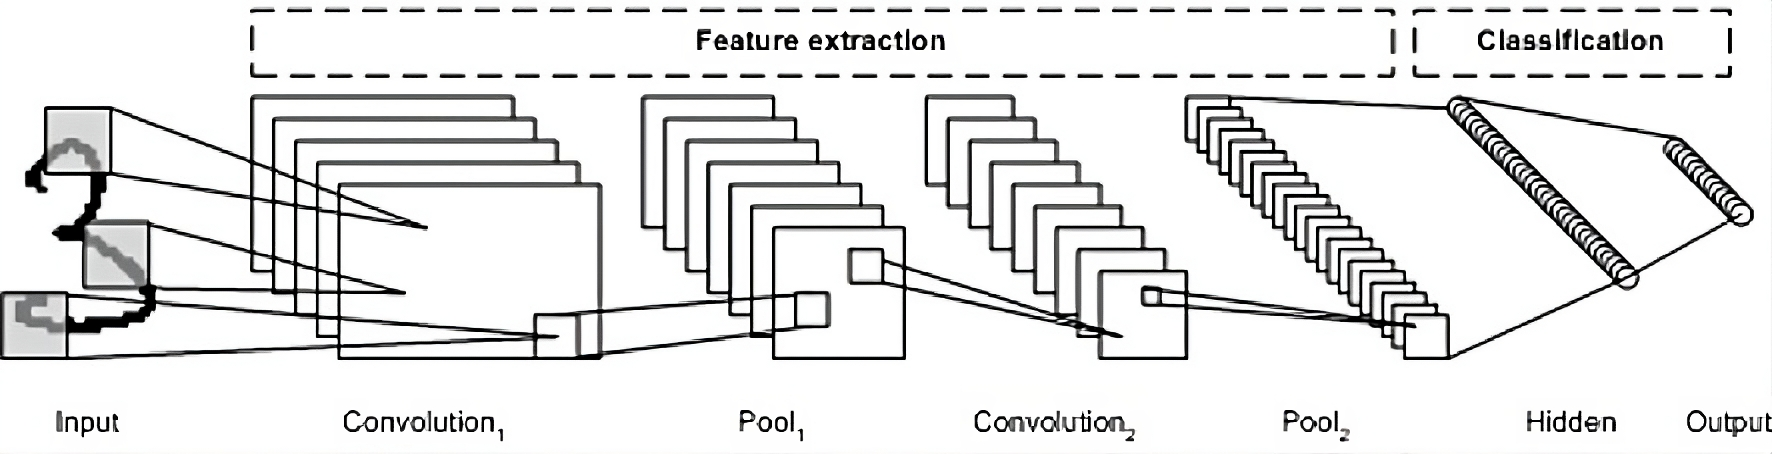
\includegraphics[width=0.9\linewidth]{Figures/CNN architecture.png} 
	\caption{LeNet CNN arhitektura \cite{IBM}}
	\label{slk:CNN-architecture}
\end{figure}

\section{Klasifikacija}

Klasifikacija je najbitniji dio procesa i može se zvati prepoznavanjem teksta u užem smislu. U početku su se OCR sustavi za klasifikaciju oslanjali na uspoređivanje znakova s unaprijed pripremljenim predlošcima (eng. \textit{template matching}), međutim, glavna manjkavost ovog pristupa osjetljivost je na promjenu fonta te šumove poput prelijevanja tinte prilikom tiska, osim očite potrebe za dodatnim ručnim radom.

Razvojem i širenjem neuronskih mreža one preuzimaju ujedno i izdvajanje značajki i njihovu klasifikaciju. Budući da neuronske mreže mogu, bez potrebe za ljudskim radom, u svojim težinama spremiti značajke na više razina apstrakcije, i, što je još bitnije, više samih značajki, nego li ljudi mogu ručno pretočiti u stroju razumljiv zapis, brzo su iskorijenile starije klasifikacijske arhitekture. \cite{Wang2012}

Za klasifikaciju znakova koriste se povratne neuronske mreže (RNN) jer omogućuju pamćenje prijašnjih ulaza te stoga mogu modelirati nizove znakova, a ne samo jedan znak poput konvolucijskih mreža.

LSTM mreže \cite{Breuel2013} (eng. \textit{long short-term memory}) vrsta su povratne mreže koje imaju dulju kratkoročnu memoriju od običnog RNN-a koji pamti samo prethodno stanje.

Transformerska arhitektura \cite{Vaswani2023} isto adresira temporalne podatke, no omogućuje paralelnu obradu ulaza što ujedno ubrzava klasifikaciju uporabom grafičkih kartica i proširuje prostor pamćenja.

\section{Naknadna obrada}

Naknadna obrada podrazumijeva metode koje djeluju na klasificirani tekst. Najčešće korištena metoda naknadne obrade jest ispravljanje riječi pomoću jezičnog modela jer značajno povećava preciznost.

Također se mogu uspoređivati rezultati različitih klasifikatora ili čak više iteracija istog klasifikatora, odlučujući na temelju glasanja koja je riječ vjerojatnija ili pak uspoređujući stupnjeve pouzdanosti transkripcije ako ih klasifikatori podržavaju. \cite{Boiangiu2016}

Osim toga, ako se prilikom faze segmentacije nisu razlučivali retci nego izravno znakovi, može se naknadno utvrditi hijerarhijski odnos teksta na slici u ovoj fazi.

%-------------------------------------------------------------------------------
\chapter{OCR starijih tekstova}
\label{pog:ocr_starijih_tekstova}

Iz specifičnosti zadatka, tj. starosti knjiga,  proizlaze određene poteškoće, naime:
\begin{itemize}
	\item Čest višak ili manjak tinte pri tisku pojedinih znakova
	\item \textcolor{red}{Zastarjela znakovlja (fontovi) s neuobičajenim znakovima} %(npr. ſ , ʒ )
	\item Otežana predobrada zbog spremanja na mikrofilmu
	\item Arhaičan jezik
	\item Neravan tisak
	\item Istrošenost i oštećenja papira
\end{itemize}

\begin{figure}[hbt]
	\centering
	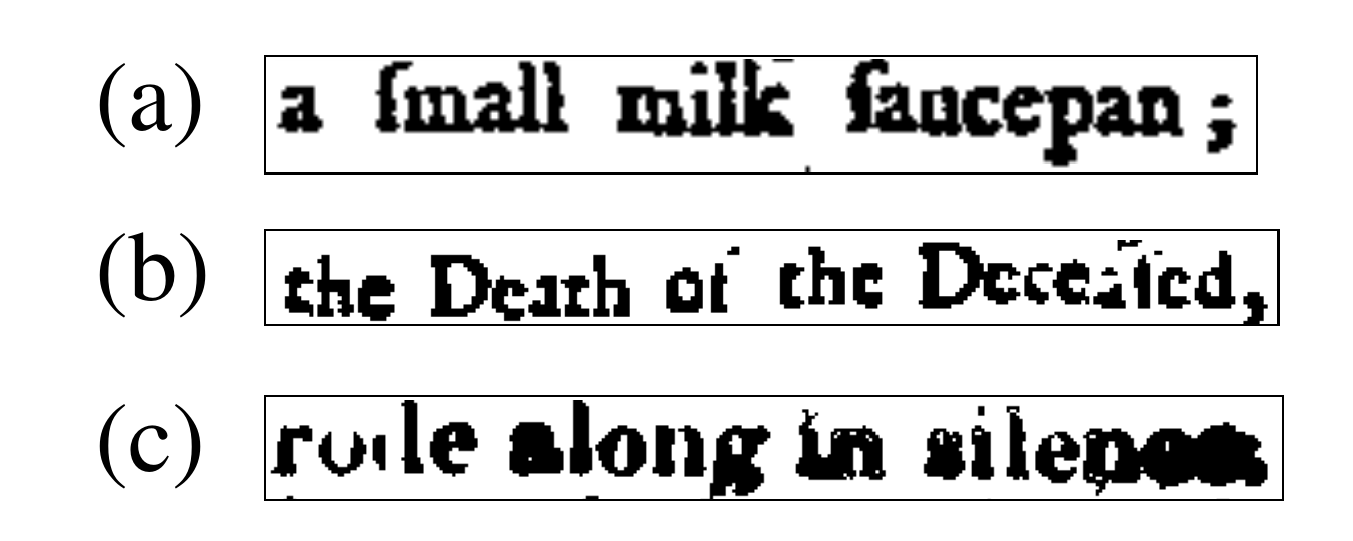
\includegraphics[width=0.6\linewidth]{Figures/historical-issues.png} 
	\caption{Isječci povijesnih dokumenta s (a) nepoznatim fontom, \\ (b) neravnim tiskom, te (c) viškom tinte. \cite{Berg2013}}
	\label{slk:historical-issues}
\end{figure}

\section{Pregled literature}

Budući da je područje rada dosta usko, ali i zahvaljujući činjenici da napredak općenitijih modernih rješenja, bilo arhitektura OCR sustava bilo obrade prirodnog jezika, u novije vrijeme zasjenjuje specijalizirane sustave, nema mnogo radova na temu transkripcije starih dokumenata.

Prvi značajan i još uvijek relevantan doprinos ujedno je i obuhvaćen ovim radom, a to su radovi u kojima je prezentiran \cite{Berg2013} i unaprijeđen Ocular \cite{Berg2014, Garrette2015, Garrette2016}, koji je razjašnjen u poglavlju \ref{pog:ocular} te se stoga ne će o njemu duljiti ovdje.


\cite{Springmann2014}
\cite{Springmann2017}


\cite{Christy2017}
\cite{Wick2018}

\textcolor{red}{U radu o Ocularu ima lista radova nekih.}


Iako se ne tiče izričtio starih dokumenata te zahtijeva nadzirano učenje, rad \textit{OCR Post Correction for Endangered Language Texts} \cite{Rijhwani2022} osobito je obećavajuć.

Naime, razvijen je model za ispravljanje transkripcije OCR sustava koji zahtijeva vrlo malo podataka za nadzirano učenje i uz to podržava učenje iz dvojezičnih ili prevedenih dokumenata. 

Za razliku od Oculara koji inkorporira jezični model u sam proces transkripcije, najveća prednost ovog rješenja jest njegova modularnost, tj. mogućnost korištenja na tekstu neovisno o OCR modelu.



%-------------------------------------------------------------------------------
\chapter{Tesseract}
\label{pog:tesseract}

Tesseract \cite{Smith2007} je najpoznatiji i najprecizniji slobodno dostupan OCR sustav opće namjene koji podržava i hrvatski jezik, a od 4. inačice temeljen je na LSTM neuronskim mrežama. U ovom poglavlju objasnit će se ugrubo Tesseractov proces prepoznavanja teksta prema zadanim postavkama.

\section{Predobrada}

Tesseract ima ugrađena tri koraka predobrade: binarizaciju, eliminaciju šuma i analizu uređenja stranica.

\subsection{Binarizacija}

Tesseract se koristi Otsuovom metodom, no ne za postavljanje jednog globalnog praga za čitavu stranicu, već rabi implementaciju Leptonica biblioteke \cite{Leptonica} koja dijeli stranicu u jednake blokove te na njima postavlja prag. Takvim pristupom nadvladavaju se varijacije u svjetlini na makro razini slike, ali se zadržava i veća resursna učinkovitost uslijed paralelizacije i izbjegavanja složenijih računa lokalnih metoda.

Za slike koje nisu više-manje dvobojne nego pate od većih nejednakosti u osvijetljenju Tesseract podržava i Sauvolinu \cite{Sauvola1997} lokalnu metodu binarizacije koja utvrđuje prag za svaki piksel slike na temelju srednje vrijednosti i standardne devijacije okolnih piksela.

\subsection{Eliminacija šuma}

Razlučivši pozadinu od ostatka prelazi se na brisanje šuma poput razlivene tinte. To se postiže pronalaskom spojenih piksela te usporedbom karakteristika nakupine s tipičnim karakteristikama teksta.

Tijekom analize razmatra se: \cite{Tesseract}

\begin{description}
	\item[Širina poteza] \hfill \\ Potezi jednolične širine vjerojatnije pripadaju znaku.
	\item[Veličina nakupina] \hfill \\ Skupine piksela koje se protežu izvan uobičajene visine retka vjerojatno nisu znakovi.
	\item[Obujmljena površina] \hfill \\ Gledajući površinu koju skupina piksela okružuje možemo procijeniti je li znak ili nije.
	\item[Broj nakupina po retku] \hfill \\ Brojeći skupine piksela u retku provjerava se omjer malih nakupina naspram skupina veličine znaka.
 	\item[Odnos među točkama] \hfill \\ Ako se detektira velik broj susjednih točaka na istoj visini ne odbacuju se već su označene kao "vodeće točke" sadržaja.
\end{description}

\subsection{Analiza uređenja stranice}

\begin{description}
	\item[Detekcija slika] \hfill \\ Funkcijom \texttt{FindImages} Tesseract pronalazi slike koje potom zanemaruje prilikom prepoznavanja teksta.
	\item[Detekcija crta] \hfill \\ Tesseract rabi Leptonicu za pronalaženje i uklanjanje crta, odnosno razdjelnih linija, na ulaznoj slici što pomaže u odvajanju teksta od grafičkih elemenata poput tablica ili obrazaca.
	\item[Analiza povezanih komponenti] \hfill \\ Ovaj korak izvodi funkcija \texttt{find\_components} koja skenira binarnu sliku piksel po piksel, označava povezane crne piksele i grupira ih u povezane komponente koje predstavljaju potencijalne znakove ili dijelove znakova.
	\item[Detekcija orijentacije i pisma] \hfill \\ Ako je ova opcija omogućena, Tesseract će provjeriti o kojem je pismu riječ (latinično, kinesko,...) i u kojem smjeru se piše (kineski se npr. može pisati odozgo prema dolje ili zdesna na lijevo).
	\item[Detekcija stupaca] \hfill \\ Koristi se ako je tekst pisan u stupcima poput novinskog članka ili znanstvenog rada.
	\item[Pronalazak redaka teksta] \hfill \\ Tesseract analizira prostorne odnose između povezanih komponenti kako bi detektirao linije teksta. Ovaj korak koristi statistički pristup temeljen na razmacima između komponenti.
\end{description}

\section{Izdvajanje značajki i klasifikacija}

 Tesseractovu arhitekturu, prikazanu na slici \ref{slk:crnn}, dobiva se združivanjem konvolucijske mreže za izdvajanje značajki te LSTM povratne mreže za klasifikaciju znakova.
 
 U procesu klasifikacije ključnu ulogu igra jezični model u kojem su spremljeni statistički uzorci jezika koje LSTM mreža koristi nakon inicijalnog raspoznavanja za upućivanje budućih pokušaja.
 
 Tesseract također sprema prilagodljive predloške koje prilagođava varijacijama fonta, kurzivu, masnopisu, podcrtavanju i sl. te razmaku među znakovima.

\begin{figure}[h!]
	\centering
	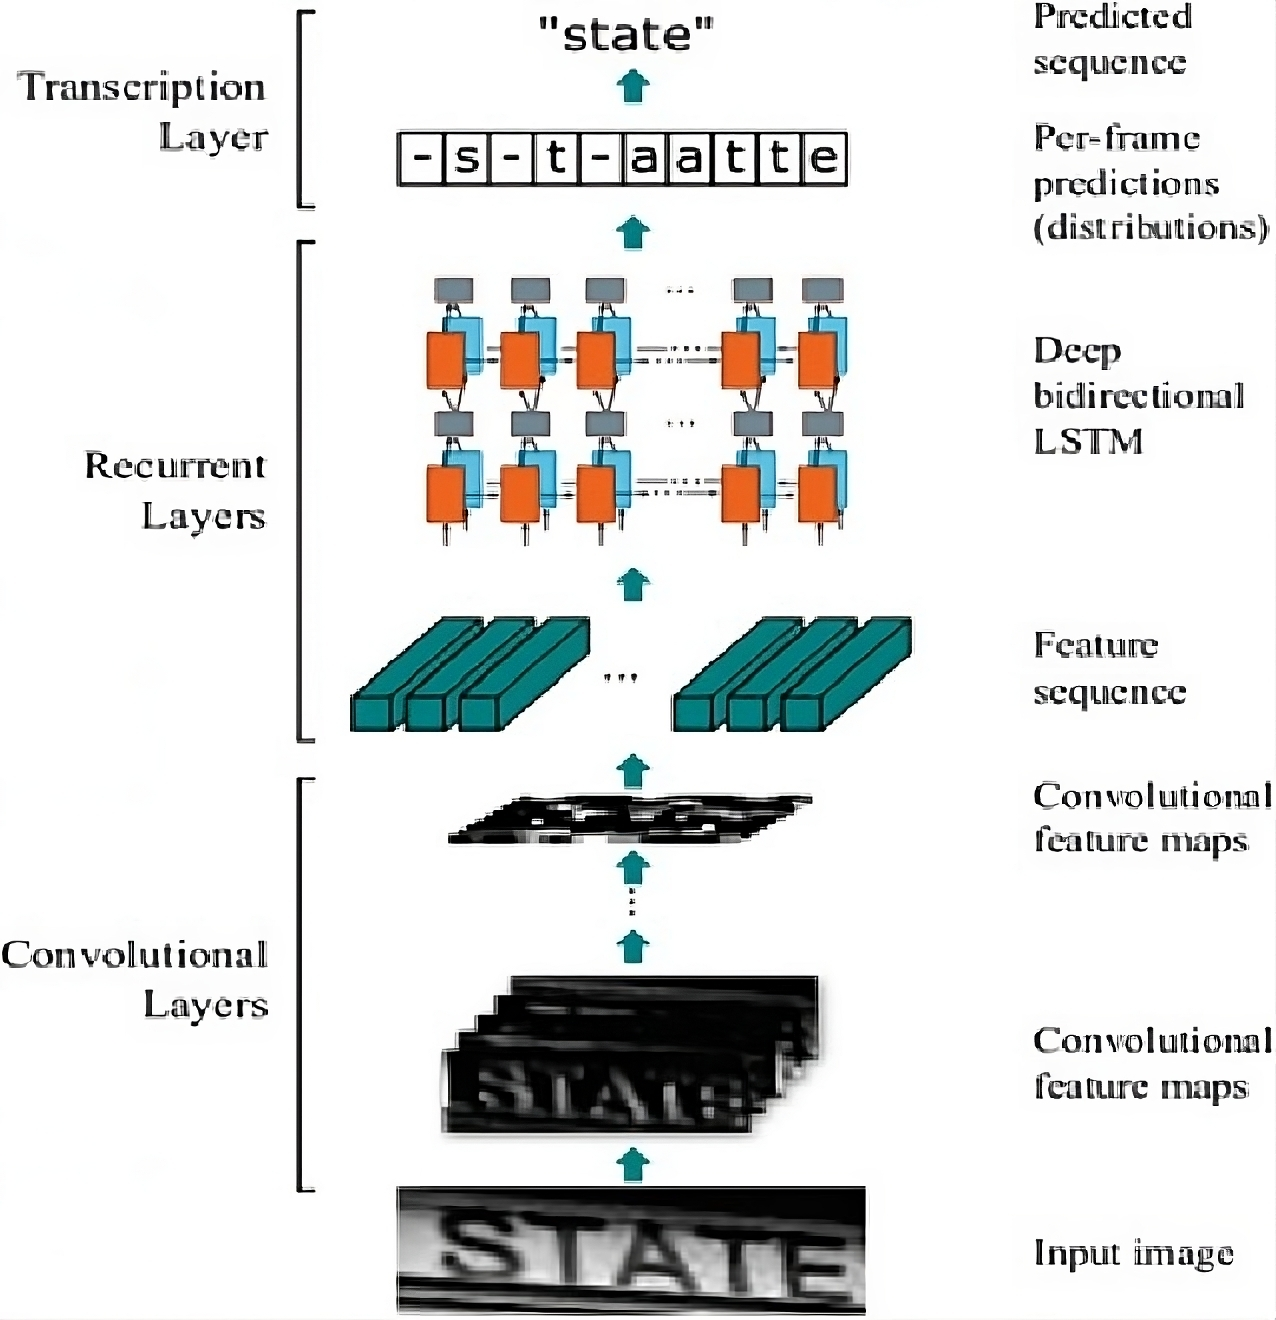
\includegraphics[width=0.7\linewidth]{Figures/CRNN-architecture.jpeg} 
	\caption{CRNN arhitektura \cite{Dharmale2023}}
	\label{slk:crnn}
\end{figure}


\section{Naknadna obrada}

Tesseract se ne koristi jezičnim modelom samo u zadnjem koraku, nego zapravo prožima čitav proces klasifikacije. Na temelju rječnika daje se prednost poznatim znakovnim nizovima, a upućen međuovisnostima jezičnog modela ispravlja riječi u skladu s kontekstom.

Konačno, Tesseract prilagođava interpunkcijske znakove i razmake pravilima jezika.



%-------------------------------------------------------------------------------
\chapter{Ocular}
\label{pog:ocular}

Ocular \cite{Berg2013} je sustav za optičko raspoznavanje teksta razvijen specifično za nenadziranu transkripciju povijesnih dokumenata, i koji je, kada je izdan i svojevremeno unaprijeđen \cite{Berg2014}, bio vrhunac tehnologije za to područje (eng. \textit{state-of-the-art}).

Njegove glavne značajke su: \cite{Ocular}

\begin{itemize}
	\item Nenadzirano učenje nepoznatih znakovlja rabeći slike ulaznog dokumenta i korpus teksta na ciljnom jeziku.
	\item Prilagođenost radu sa šumovitim dokumentima.
	\item Podrška za višejezične dokumente.
	\item Nenadzirano učenje ortografskih varijacija uslijed arhaičnog pravopisa.
	\item Istovremen ispis doslovnog teksta i normaliziranog oblika (prilagođenog standardnom jezku).
\end{itemize}

U \ref{pog:ocr_uvod} poglavlju spomenuta je klasifikacijska metoda uspoređivanja predložaka čiji je glavni nedostatak neprilagodljivost na različita znakovlja.

Ocular nadilazi tu poteškoću gradeći model znakovlja dinamički, tj. po potrebi za svaki dokument, te ne uspoređuje ulazni znak izravno s predloškom, već na temelju naučenog modela, uzimajući u obzir kontekst, nagnuće teksta, količinu tinte i šum, generira znak koji potom uspoređuje s pikselima ulaznog znaka.

To postiže četirima generativnim probabilističkim modelima koji predstavljaju aspekte procesa tiskanja: jezični model, slovoslagarski ili tipografski model, koji uključuje model tinte, te model šuma, koji združeni tvore skriveni polu-Markovljev model (HSMM).

Međuovisnosti ulaza i modela određuje sljedeća formula, \cite{Berg2013} gdje \textit{E} predstavlja tekst, \textit{X} piksele ulazne slike, \textit{T} raspored znakova na slici, a \textit{R} aspekte otiskivanja tinte:

\[
\begin{aligned}
	P(E, T, R, X) &= P(E) & \text{[Jezični model]} \\
	&\cdot P(T | E) & \text{[Slovoslagarski model]} \\
	&\cdot P(R) & \text{[Model tinte]} \\
	&\cdot P(X | E, T, R) & \text{[Model šuma]}
\end{aligned}
\]

\section{Jezični model}

Jezični model jest Kneser-Neyev uglađeni znakovni \textit{n}-gramski model \cite{Kneser1995} koji se uči na korpusu teksta u ciljnom jeziku. Specifičnost ovog modela, koja ga razlikuje od uobičajenih NLP modela, je da nema zaustavni znak, nego tretira cijeli redak kao jednu cjelinu, sadržavala ona jednu rečenicu ili pak više njih.

Blisko povezan s jezičnim modelom pojam je veličine snopa (eng. \textit{beam size}) pretraživanja skupa stanja. Naime, prilikom treniranja modela znakovlja, a i same transkripcije, na temelju jezičnog modela generiraju se najvjerojatniji slijedovi znakova, koji se potom uspoređuju s ulazom i od kojih se odabire najsličniji.

Veličina snopa označava jednostavno broj tih nizova koji će se uzeti u obzir. \cite{Berg2014} Veći snop će produljiti vrijeme izvršavanja, a i prevelik snop može dovesti do prenaučenosti.


\section{Slovoslagarski model}

	
Slovoslagarstvo (eng. \textit{typesetting}) u kontekstu mehaničkog tiskanja podrazumijeva postavljanje glifova znakova prikladno razmaknute na traku za tiskanje.

Ocularov generativni model radi vrlo sličnu stvar. \ref{fig:typesetting-model} Prvo generira širinu glifa $g_i$, zatim lijevi razmak $l_i$ te desni razmak $r_i$, koji naravno ovise o prepoznatom znaku $e_i$.

\begin{figure}[H]
	\centering
	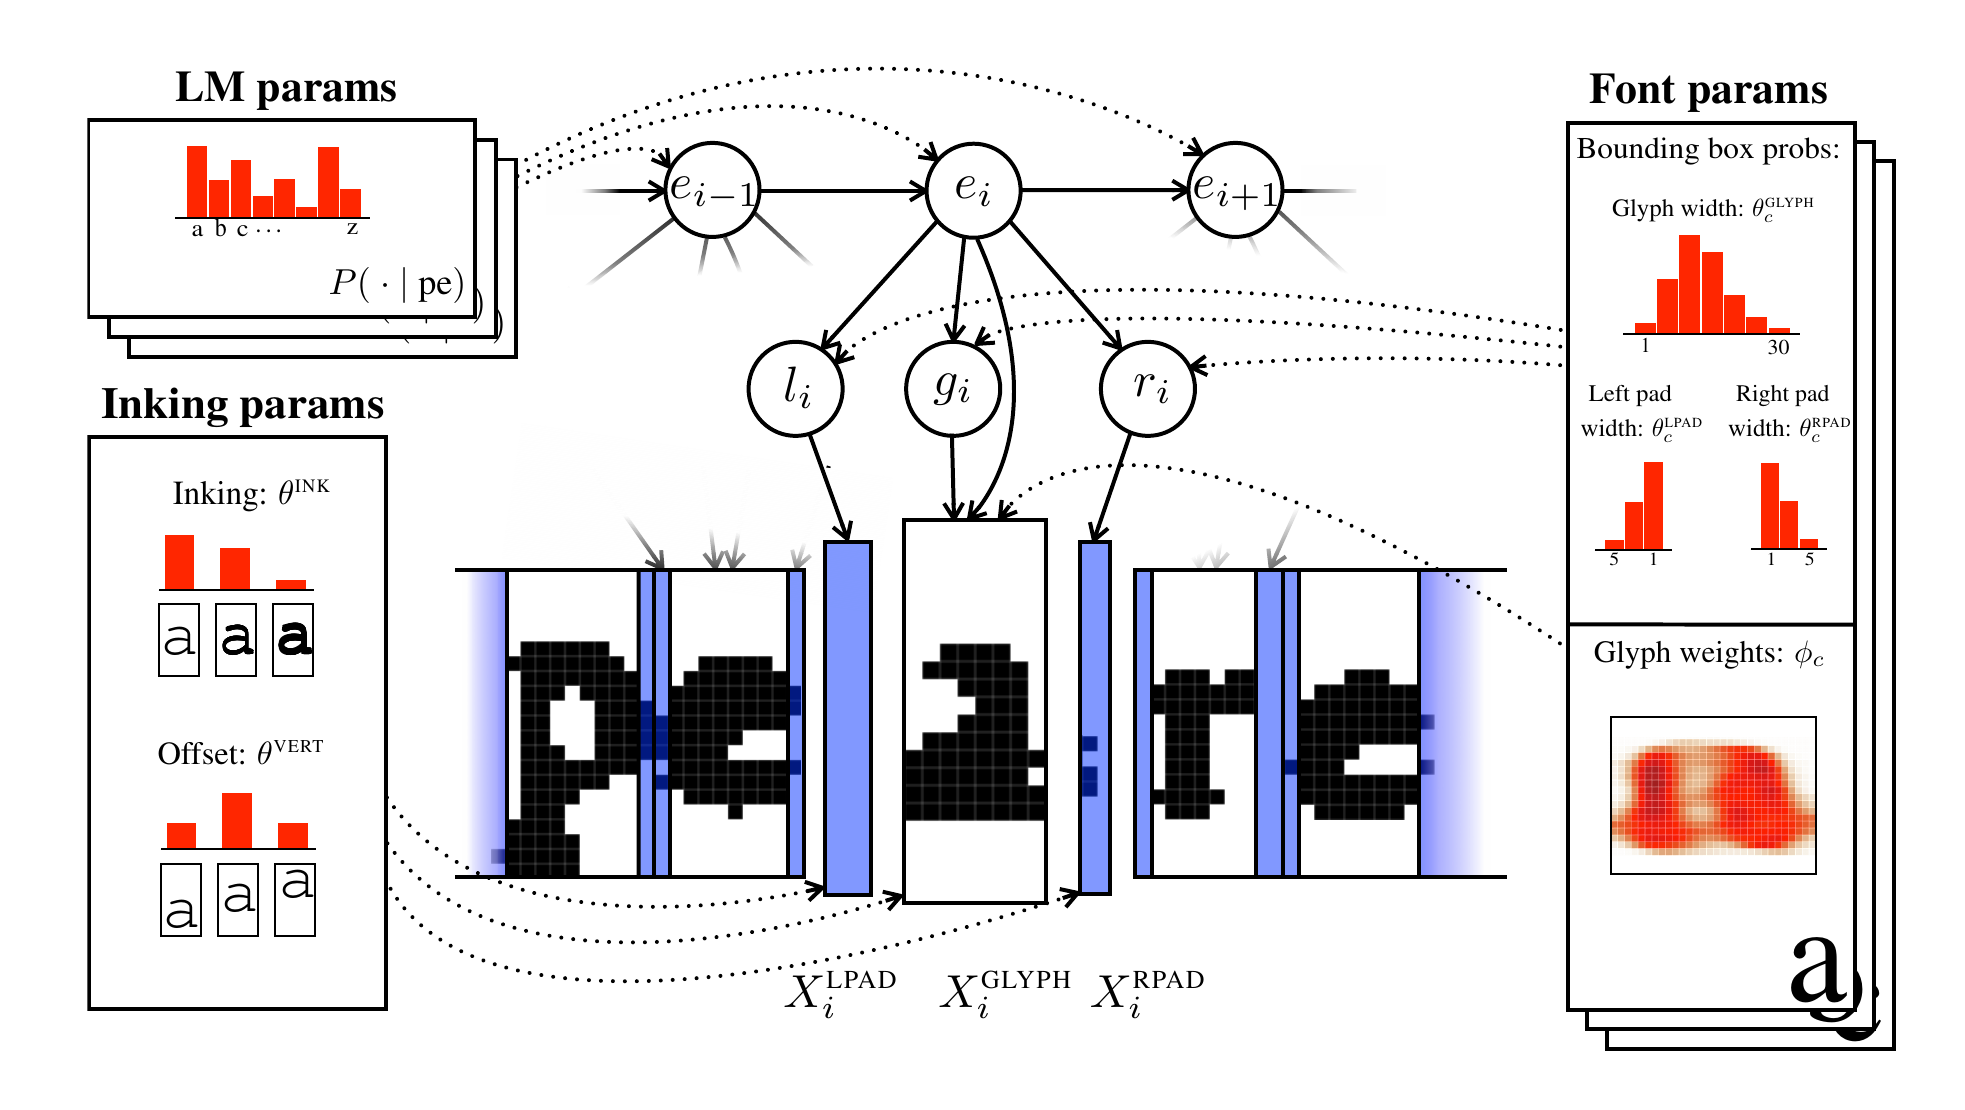
\includegraphics[width=1.0\linewidth]{Figures/typesetting-model.png} 
	\caption{Stohastički proces generiranja glifa znaka \cite{Berg2013}}
	\label{fig:typesetting-model}
\end{figure}


\subsection{Model tinte}

\setlength{\parskip}{0pt}
\begin{multicols}{2}	
	% First column
	Kako bi generirani znak bio sličan ulaznom potrebno je odabrati prikladnu količinu tinte, ali i vertikalni pomak.
	
	To postiže generiranjem količine tinte za raspodjelu po pikselima $d_i$ te pomak od dna $v_i$.
	
	Ove vrijednosti obično ne ovise o vrsti znaka te su stoga tako modelirane i u stohastičkim modelima.
	
	\section{Model šuma}
	
	Model šuma simulira degradaciju slike koja nastaje tijekom procesa tiskanja dodavanjem šuma u obliku neovisnog bijeljenja piksela prema Gaussovoj distribuciji.
	
	% Second column
	\columnbreak
	\begin{figure}[H]
		\centering
		\vspace{10pt}
		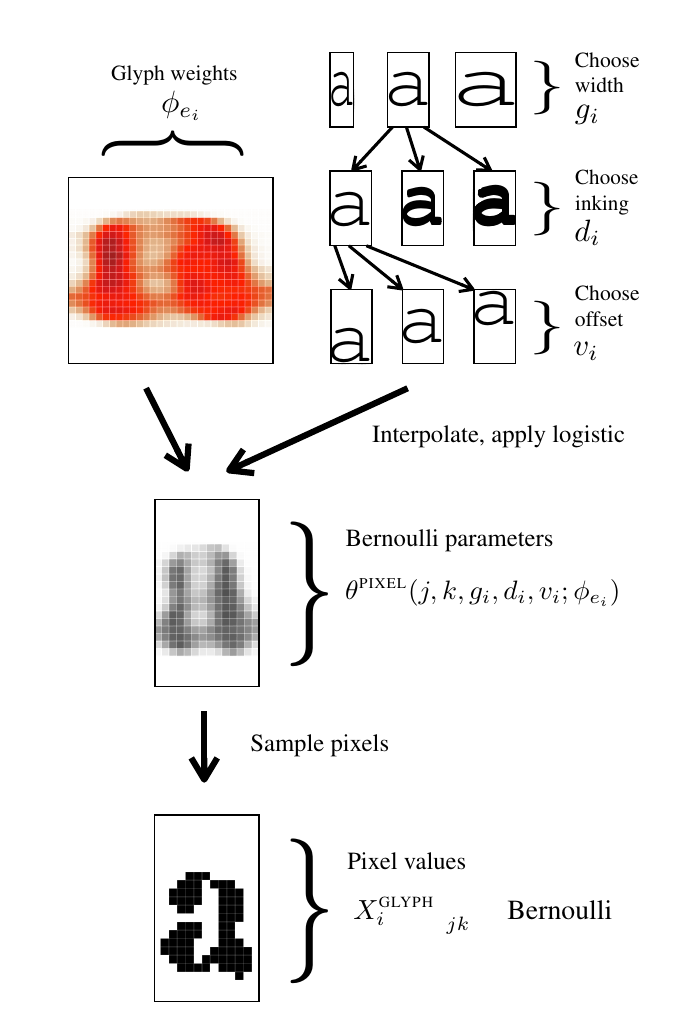
\includegraphics[width=0.9\linewidth]{Figures/inking-model.png} 
		\caption{Stohastički proces zacrnjivanja piksela glifa \cite{Berg2013}}
		\label{fig:inking-model}
	\end{figure}
	
\end{multicols}

Na kraju zadržava najcrnje piksele kao što je učinjeno na ulazu tijekom binarizacije.








%-------------------------------------------------------------------------------
\chapter{Metodologija}
\label{pog:metodologija}

Ključan dio razvoja boljeg rješenja evaluacija je preciznosti Tesseracta i Oculara. U tu svrhu potreban je ispitni skup podataka prilagođen ograničenjima sustava. 

Zatim treba prikupiti podatke za treniranje Oculara i namjestiti njegove hiperparametre da daju zadovoljavajuće rezultate, što će zapravo biti najznačajniji dio rada.


\section{Ispitni skup podataka}

Budući da Tesseract ima ugrađenu predobradu slika, radi pravednije usporedbe same klasifikacije teksta izabrani su već obrađeni dokumenti:

\begin{itemize}
	\item Fra Jozo Garić, biskup – Korizmena okružnica (1932.) \ref{slk:korizmena}
	\item Sv. Petar Kanizije – Summa nauka christianskoga (1583.) \ref{slk:summa}
\end{itemize}

Korizmena okružnica korištena je za sva ispitivanja osim za isprobavanje ortografskih mogućnosti gdje je izabrana \textit{Summa} kao primjer zahtjevnog ulaza za sustav.

\begin{figure}[H]
	\centering
	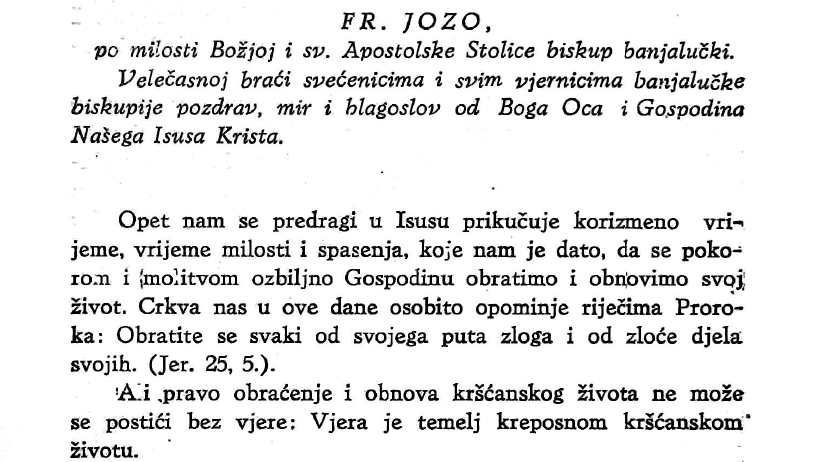
\includegraphics[width=1.0\linewidth]{Figures/korizmena.png} 
	\caption{Izvadak iz \textit{Korizmene okružnice}}
	\label{slk:korizmena}
\end{figure}

\begin{figure}[H]
	\centering
	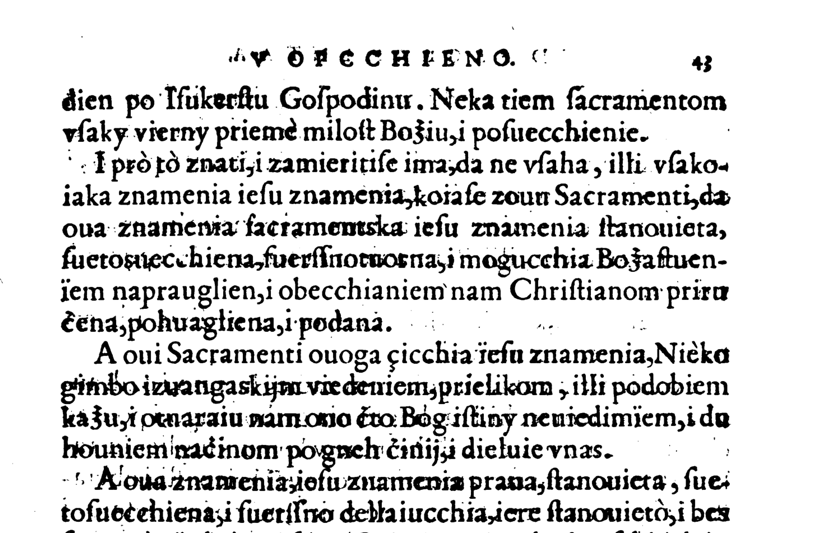
\includegraphics[width=1.0\linewidth]{Figures/summa.png} 
	\caption{Izvadak iz \textit{Summe nauka christianskoga}}
	\label{slk:summa}
\end{figure}

Oba sustava imaju određena ograničenja na ulaze: 

Ocular radi jedino s PDF dokumentima zastarjele verzije 1.4 te ih je stoga bilo potrebno pretvoriti u taj format. Za to je korišten Ghostscript, \cite{Ghostscript} slobodno dostupan alat otvorenog koda. 

Tesseract pak radi jedino na slikama te je zato bilo potrebno ekstrahirati ih iz PDF-a prije prepoznavanje teksta. Ovdje je zgodno napomenuti da treba paziti da se prilikom pretvorbe ne smanji DPI rezolucija jer to ima poguban utjecaj na preciznost.

\section{Mjere uspješnosti}

Za uspoređivanje znakovnih nizova najčešće korištena mjera uspješnosti je \textbf{Levenshteinova udaljenost} koja bilježi broj potrebnih zamjena, brisanja ili umetanja znakova da bi se iz jednog niza dobio drugi. \cite{Levenshtein1965}

Budući da ta mjera ovisi o duljini teksta, dijeljenjem Levenshteinove udaljenosti ukupnim brojem znakova dobivamo \textbf{stopu pogreške za znakove} (eng. \textit{Character Error Rate}). Obično se dobrom vrijednošću smatra 1-2\%.

\textbf{Stopa pogreške za riječi} (eng. \textit{Word Error Rate}) dobiva se uzimanjem riječi za najmanju jedinicu zamjene pri računanju Levenshteinove udaljenosti, tj. ako su jedan ili više znakova u riječi pogrešni čitava riječ broji se kao pogrešna, te dijeljenjem te udaljenosti s ukupnim brojem riječi.

\section{Naknadna obrada}

\textcolor{red}{\textit{Tesseract zamjena ',,' (dva zareza) s " (ravni navodnici)}}

Za Ocular duge crte u -

Jednostavno se može naknadno utvrditi treba li biti duga ili kratka crta.

%-------------------------------------------------------------------------------
\chapter{Optimizacija Oculara}
\label{pog:optimizacija_oculara}

Za razliku od Tesseracta, Ocular nije univerzalno primjenjiv za različite jezike i znakovlja već je potrebno naučiti jezični model, za koji je potreban korpus teksta na ciljnom jeziku, te model fonta, koji se gradi na temelju slika čiji će tekst kasnije prepoznavati. U ovom poglavlju, koje predstavlja i glavni dio rada, provest će se optimizacija Ocularovih hiperparametara.

\section{Jezični model}

Pri izgradnji skupa podataka za trening jezičnog modela najrelevantnije su dvije stavke: broj podataka i tematika teksta.

U izvornom radu pokazano je kako model malo precizniji (4 WER postotna boda) na dokumentima čija je tematika pokrivena u jezičnom modelu. Budući da je sustav namijenjen starijim knjigama, od kojih je dobar dio vjerske tematike, uključeno je Sveto Pismo i druge duhovne knjige pored novijeg i starijeg štiva koje doprinosi većoj raznolikosti izričaja i opsežnijem rječniku.
\cite{Berg2013}

U daljnjim eksperimentima korišten je jezični model treniran na tekstovima javno dostupnih knjiga, poput djela Augusta Šenoe, Marije Jurić-Zagorke, Charlesa Dickensa i sl. (7.5 milijuna riječi) uz Šarićev prijevod Svetog Pisma (670k riječi) i još 11 knjiga vjerske tematike (500k riječi). 

Ukupan broj riječi odabranog skupa podataka od 8.7 milijuna usporediv je sa skupom podataka korištenim u izvornom radu koji ih ima 10 milijuna.

\subsection{Veličina skupa podataka}

Ispitani su i podskupi odabranog ali i veći skupovi podataka, temeljeni na prethodno navedenom uz dva tipa proširenja: stranom i domaćom beletristikom (11.6 milijuna riječi) te tekstovima vjerske tematike (6 milijuna riječi). 

Nažalost, dodatak beletristike dovodio je do neizbježnog neuspjeha treninga te je stoga ispitano samo proširenje vjerskim štivom.

Tekstovi vjerskih knjiga nisu bili lektorirani nego nesavršeni proizvodi prepoznavanja teksta, a uključeni su svejedno kako bi se ispitalo doprinosi li kvantiteta potencijalno više od kvalitete ako greške nisu značajne.

Kako je vidljivo iz tablice \ref{tab:lm_performance}, povećanje skupa podataka ipak je dovelo do smanjenja preciznosti. Ručnom provjerom lako se uviđa kako su greške iz jezičnog modela utjecale na ispis.

Primjerice, prvotni jezični model ispravno prepoznaje riječ \texttt{katekizam}, dok ju prošireni zamijenjuje nizom \texttt{katalo sam}, s tim da se niz \texttt{katalo} pojavljuje samo jednom u proširenom skupu podataka.

Očigledno, Ocularov jezični model nije robustan na greške u skupu podataka čak i kad se pojavljuju samo jednom, što je razumljivo, jer je poželjno da svaka viđena riječ postane dio vokabulara.

Ipak, pomalo je iznenađujuće da je \texttt{katalo} nadjačalo riječ koja se pojavljuje 80 puta u skupu podataka. Međutim, čini se kako je do toga došlo zbog kombinacije s nizom \texttt{sam} koji se pojavljuje preko 57 tisuća puta.



\bgroup
\def\arraystretch{1.25}
\begin{table}[h]
	\centering
	\begin{tabular}{|c|c|c|}
		\hline
		 \textbf{Jezični model} & \textbf{CER} & \textbf{WER} \\ \hline
		 Izvorni & 1.05 & 2.74 \\ \hline
		 Izvorni + OCR vjerskih knjiga & 1.59 & 3.64 \\ \hline
	\end{tabular}
	\caption{Uspješnost povećanja jezičnog modela}
	\label{tab:lm_performance}
\end{table}
\egroup



\subsection{Veličina snopa}

S obzirom na to da veći jezični model podrazumijeva više mogućih kombinacija riječi, povećanje snopa ispitivanih riječi u skrivenom Markovljevom modelu postaje potencijalno presudno kako bi točna riječ bila pronađena.

Ipak, kako je vidljivo iz donje tablice \ref{tab:7.2}, povećanje snopa nije dovelo do poboljšanja niti pri treningu modela fonta niti prilikom transkripcije.

\bgroup
\def\arraystretch{1.25}
\begin{table}[h]
	\centering
	\begin{tabular}{|c|c|c|c|c|}
		\hline 
		\multicolumn{2}{|c|}{\textbf{Veličina snopa}} & \multicolumn{1}{|c|}{\multirow{2}{*}{\textbf{CER}}} & \multicolumn{1}{|c|}{\multirow{2}{*}{\textbf{WER}}} \\ \cline{1-2}
		
		\textbf{Trening}  & \textbf{Transkripcija}  & \multicolumn{1}{|c|}{}  & \multicolumn{1}{|c|}{}  \\ \hline
		10  & 10 &  2.03 & 3.58  \\ \hline
		40 & 40 &  1.59 & 3.64   \\ \hline
		50 & 50 &  \textbf{1.05} & \textbf{2.74}   \\ \hline
		40 & 120 & 1.81 & 3.77   \\ \hline
		120 & 50 & 2.21 & 5.04 \\ \hline        
		120 & 120 & 2.29 & 5.78 \\ \hline                                             
	\end{tabular}
	\caption{Usporedba uspješnosti prema veličini snopa}
	\label{tab:7.2}
\end{table}
\egroup

Rezultati impliciraju kako je bolje ne ispraviti prepoznati znakovni niz ako predloženi ispravak nije među prvih pedeset predloženih. To može biti do grešaka u skupu podataka za jezični model, gdje veći snop obuhvati i rijetke pogrešne, ali slične nizove ispravljanome. 

Općenitije gledano, povećanje snopa pretraživanja prostora stanja podržava "pamćenje" više informacija i stoga dovodi do prenaučenosti, kao i prekomjerno povećanje neuronske mreže. Drugim riječima, veća veličina snopa podložnija je utjecaju šuma. 

Tomu u prilog ide, primjerice, zamjena rijetkog niza \texttt{vjere:}, koji se pojavljuje 4 puta u skupu podataka, riječju \texttt{vjetar}, koja se pojavljuje 897 puta. 

\section{Model znakovlja}

\begin{multicols}{2}
	
Budući da se Ocularova klasifikacija zasniva na generiranju znakova na temelju modela znaka opisanog matricom vjerojatnosti, \ref{slk:matrica} ključno je te vjerojatnosti pomno odrediti.

Rezultati ispitivanja optimalnog broja faza treninga modela fonta vidljivi su u tablici \ref{tab:7.3}  Suprotno očekivanjima, ponovno treniranje na prve dvije stranice nije povećalo preciznost.

	\columnbreak
	
\begin{figure}[H]
	\centering
	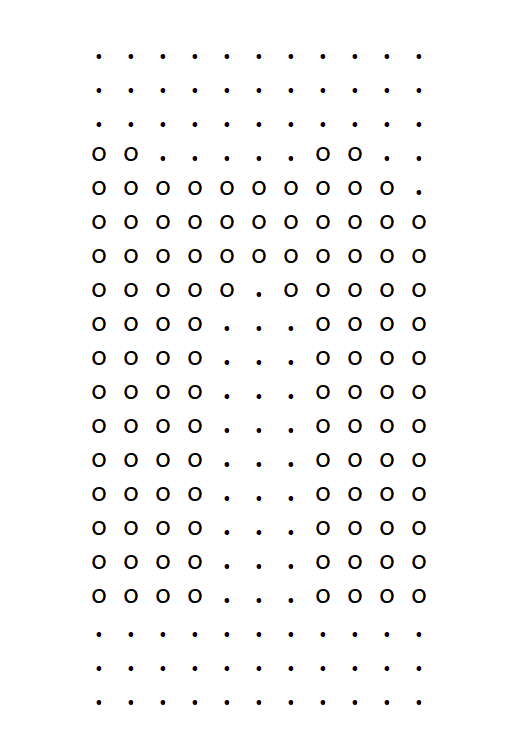
\includegraphics[width=0.6\linewidth]{Figures/letter-matrix.png} 
	\caption{Matrica vjerojatnosti za slovo \texttt{n}. Svaki kružić predstavlja vjerojatnost da je piksel zacrnjen.}
	\label{slk:matrica}
\end{figure}

\end{multicols}



\bgroup
\def\arraystretch{1.25}
\begin{table}[h]
	\centering
	\begin{tabular}{|c|c|c|c|c|}
		\hline
		\multirow{2}{*}{\textbf{Iteracije treninga}} & \multicolumn{2}{c|}{\textbf{Veličina snopa}} & \multicolumn{1}{c|}{\multirow{2}{*}{\textbf{CER}}} & \multicolumn{1}{c|}{\multirow{2}{*}{\textbf{WER}}} \\ \cline{2-3}
		
		& \textbf{Trening}  & \textbf{Transkripcija}  & \multicolumn{1}{c|}{}  & \multicolumn{1}{c|}{}  \\ \hline
		\multirow{2}{*}{3x3 stranice} & 10 & 10 & 2.03 & 3.58  \\ \cline{2-5}
		 		& 50  & 50 & \textbf{1.05} & \textbf{2.74}   \\ \hline
		3x3 str. + 2x2 str. & 50 & 50 & 1.19 & 2.9 \\ \hline                                              
	\end{tabular}
	\caption{\textcolor{red}{Lorem ipsum}}
	\label{tab:7.3}
\end{table}
\egroup


Gledajući pobliže, uspješnost opada na jednoj od dvije stranice koje su prošle dodatne dvije iteracije treninga, a na drugoj se povećava. \ref{tab:pages5and6} Radi se o razlici od nekoliko znakova te se stoga ne može zaključiti poboljšava li se barem uspješnost na dotreniranim stranicama kao kod školskog primjera prenaučenosti.


\bgroup
\def\arraystretch{1.25}
\begin{table}[hbt]
	\centering
	\begin{tabular}{|c|c|c|c|}
		\hline
		\textbf{Ispitivana stranica} & \textbf{Model znakovlja} & \textbf{CER} & \textbf{WER} \\ \hline
		\multirow{2}{*}{str. 5.} & 3x3 & \textbf{0.73} & \textbf{1.49} \\ \cline{2-4}
								 & 3x3+2x2 & 1.20 & 3.08 \\ \hline
		\multirow{2}{*}{str. 6.} & 3x3 & 1.17 & 3.16 \\ \cline{2-4}
								 & 3x3+2x2 & \textbf{0.95} & \textbf{1.46} \\ \hline
	\end{tabular}
	\caption{}
	\label{tab:pages5and6}
\end{table}
\egroup

\FloatBarrier

\section{Ispitivanje ortografskih mogućnosti}

\textcolor{red}{Rad na Summi. Loši rezultati i malo podataka. Spominjati ili ne?}

Kako bi uspješno prepoznavali arhaične ortografske varijacije, u izvornom radu \cite{Garrette2016} pretvorbom suvremenih tekstova, na temelju pravila koja su definirali jezikoslovci, konstruiran je skup podataka s arhaičnim ortografskim varijacijama.

U ovom odjeljku ukratko se demonstrira kako je za uspješnu transkripciju vrlo starih dokumenata arhaičnog jezika potreban značajniji trud od jednostavnog treniranja modela na korpusu suvremenog teksta.


\subsection{Jezični model}

Moglo bi se očekivati da će veći rječnik više doprinijeti uspjehu na tekstovima s dotad manjom preciznošću prepoznavanja, kao što je \textit{Summa nauka christianskoga}, međutim, povećanje skupa podataka nije dovelo do značajnog poboljšanja u preciznosti, ali je značajno usporilo trening i transkripciju.

\bgroup
\def\arraystretch{1.25}
\begin{table}[h]
	\centering
	\begin{tabular}{|c|c|c|c|}
		\hline
		\textbf{Ispitivani dokument} & \textbf{Jezični model} & \textbf{CER} & \textbf{WER} \\ \hline
		\multirow{2}{*}{Summa nauka christianskoga} & Izvorni & 17.67 & 66.79 \\ \cline{2-4}
		& Izvorni + OCR vjerskih knjiga & 16.52 & 64.64 \\ \hline
	\end{tabular}
	\caption{Usporedba uspješnosti jezičnih modela}
	\label{tab:ortography_performance}
\end{table}
\egroup

Minimalno poboljšanje vidljivo u tablici \ref{tab:lm_performance} za \textit{Summu} u granicama je slučajnosti, osobito uzevši u obzir da je za tu knjigu ispitivana samo jedna stranica (iako je trening modela fonta bio na 6) naspram 12 za \textit{Korizmenu okružnicu}.

%-------------------------------------------------------------------------------
\chapter{Sinteza rješenja}
\label{pog:sinteza_rješenja}

Budući da je izuzev ispuštanja određenih redaka Ocular točniji od Tesseracta ovdje se predlaže jednostavan sustav glasanja kojim je Ocularova manjkavost otklonjena bez gubitka preciznosti.

Algoritam glasanja čita redak po redak Tesseractov ispis i traži odgovarajući redak Ocularovog ispisa na temelju sličnosti izračunate pomoću Levenshteinove udaljenosti. Ako pronađe dovoljno sličan redak odabire ga kao izlaz, inače preferira Tesseractov ispis.

\begin{figure}[h]
	\centering
	\begin{adjustwidth}{1cm}{1cm}
		\begin{lstlisting}
			for t_line in tesseract_output:
				for c_line in ocular_output:
					distance = Levenshtein.distance(t_line, c_line)
					if distance < threshold * len(t_line):
						output.append(c_line)
					break
				output.append(t_line)
		\end{lstlisting}
	\end{adjustwidth}
	\caption{Algoritam glasanja predstavljen Python kodom}
	\label{fig:python_code}
\end{figure}

Suradnjom dvaju modela dobiva se bolji rezultat kao što je vidljivo u tablici \ref{tab:system_performance}.

\bgroup
\def\arraystretch{1.25}
\begin{table}[h]
	\centering
	\begin{tabular}{|c|c|c|c|}
		\hline
		\textbf{OCR sustav} & \textbf{Pojedinosti} & \textbf{CER} & \textbf{WER} \\ \hline
		\multirow{2}{*}{Ocular} & & 8.83 & 10.94 \\ \cline{2-4}
								& Zanemareni retci s CER>20 & 1.05 & 2.74 \\ \hline
		Tesseract & & 1.52 & 3.77 \\ \hline
		Predložen sustav & & \textbf{0.96} & \textbf{2.48} \\ \hline
	\end{tabular}
	\caption{Uspješnosti sustava}
	\label{tab:system_performance}
\end{table}
\egroup

A na slici \ref{fig:compare} vidljiv je primjer transkripcije za najzahtjevniju stranicu ispitnog skupa.

% Line 1
\begin{figure}[H]
	\centering
	\begin{minipage}{0.85\linewidth}
		\fbox{\texttt{\small Da griješan život vodi do otpada od vjere, svjedoči nam}}
		\vspace{0.5em}
		
\includegraphics[width=\linewidth]{Figures/korizmena9/1.png}
	\end{minipage}
	\centering
	\begin{minipage}{0.85\linewidth}
		\fbox{\texttt{\small pov\textcolor{red}{la}st svih vremena. U 16. stoljeću otpadoše milij\textcolor{red}{u}ni od Ka-}}
		\vspace{0.5em}
		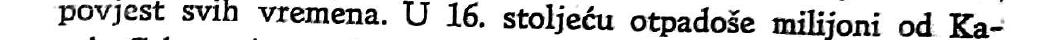
\includegraphics[width=\linewidth]{Figures/korizmena9/2.png}
	\end{minipage}
	\begin{minipage}{0.85\linewidth}
		\texttt{\fbox{\small \textcolor{red}{r}ol Crkve. A uzrokom tome bio je samo slobodan i razudan}}
		\vspace{0.5em}
		
\includegraphics[width=\linewidth]{Figures/korizmena9/3.png}
	\end{minipage}
	\begin{minipage}{0.85\linewidth}
		\texttt{\fbox{\small  život. Nova nauka \textcolor{red}{o}ga\textcolor{red}{n}jala je taštini i udobnosti. Jer se više}}
		\vspace{0.5em}
		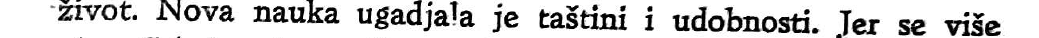
\includegraphics[width=\linewidth]{Figures/korizmena9/4.png}
	\end{minipage}
	\begin{minipage}{0.85\linewidth}
		\texttt{\fbox{\small nisu Crkvi pokorava\colorbox{pink}{\tiny}i\colorbox{pink}{\tiny} tražili su sami sebi vjeru, te su mogli}}
		\vspace{0.5em}
		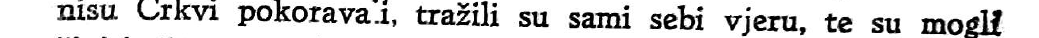
\includegraphics[width=\linewidth]{Figures/korizmena9/5.png}
	\end{minipage}
	\begin{minipage}{0.85\linewidth}
		\texttt{\fbox{\small činiti, što su god htjeli. Ta je nova vjera pustila uzde svim }}
		\vspace{0.5em}
		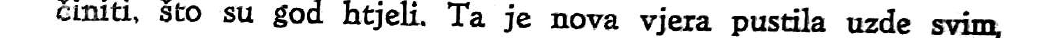
\includegraphics[width=\linewidth]{Figures/korizmena9/6.png}
	\end{minipage}
	\begin{minipage}{0.85\linewidth}
		\texttt{\fbox{\small strastima, otvorila je vrata\colorbox{pink}{\tiny} oh\textcolor{red}{lo}sti, taštini, pohlepi, otimačini}}
		\vspace{0.5em}
		
\includegraphics[width=\linewidth]{Figures/korizmena9/7.png}
	\end{minipage}
	\begin{minipage}{0.85\linewidth}
		\texttt{\fbox{\small i svim drugim grijesima. Nije čudo, što su staru vjeru s njenim }}
		\vspace{0.5em}
		
\includegraphics[width=\linewidth]{Figures/korizmena9/8.png}
	\end{minipage}
	\begin{minipage}{0.85\linewidth}
		\texttt{\fbox{\small strogim propisima odbacili, a prihvati\colorbox{pink}{\tiny}i novu, u kojoj se moglo}}
		\vspace{0.5em}
		
\includegraphics[width=\linewidth]{Figures/korizmena9/9.png}
	\end{minipage}
	\begin{minipage}{0.85\linewidth}
		\texttt{\fbox{\small lahko živjeti.\\}}
		\vspace{0.5em}\\
		
\includegraphics[width=\linewidth]{Figures/korizmena9/10.png}
	\end{minipage}
	\caption{Transkricpija isječka najlošije stranice.}
	\label{fig:compare}
\end{figure}



%--- ZAKLJUČAK / CONCLUSION ----------------------------------------------------
\chapter{Zaključak}
\label{pog:zakljucak}

Usprkos općenitom napretku OCR sustava, suvremena rješenja imaju određene manjkavosti praktične naravi. Poglavito to je potreba za skupovima označenih podataka, a često i velikim jezičnim korpusom kako bi se prilagodila novom jeziku.

Tesseract pak predstavlja jednostavno, gotovo rješenje no uz nezadovoljavajuća preciznost. Ocular, s druge strane, izbjegavajući zahtjeve nadziranog učenja te nadilazeći Tesseractovu preciznost na starim dokumentima, ipak pati od svojih problema.

Prvenstveno to je resursno zahtjevan i dugotrajan proces učenja i transkripcije (min. po str.), i to usprkos OpenCL paralelizaciji, koja je korištena umjesto bolje CUDA paralelizacije, jer se potonju, notornu za lošu kompatibilnost s Java-om, nije uspjelo omogućiti.

Osim toga, često ispušta kraće retke, što je za cjelovito rješenje neprihvatljivo te je stoga Ocularov ispis ispravljen Tesseractovim.

Dodatno poboljšanje preciznosti predloženog sustava moglo bi se postići složenijim sustavom glasanja temeljenom na detaljnijoj analizi grešaka pojedinih modela.

Primjerice, uzevši u obzir kako Ocularov jezični model djeluje nad retcima umjesto nad rečenicama, očekivalo bi se da čini više grešaka na prvoj riječi retka nego Tesseract, osobito uslijed hifenacije.

S druge strane, čini se kako Tesseract češće prepoznaje interpunkciju kada treba i kada ne treba uslijed većeg oslanjanja ne predobradu naspram jezičnog modela te bi u tom slučaju preferiranje Ocularove interpunkcije poboljšalo uspješnost.

Na žalost za Ocular, ali na sreću optičkog raspoznavanja znakova, modernije arhitekture pružaju sve bolje rezultate, a i razvojem velikih jezičnih modela dolazi do sve veće konvergencija OCR-a i obrade prirodnog jezika.

Imajući taj trend u vidu, budućnost transkripcije povijesnih dokumenata nazire se u naknadnoj obradi teksta, koja bi pružala svevremensko rješenje neovisno o klasifikacijskoj arhitekturi.



%--- LITERATURA / REFERENCES ---------------------------------------------------
% Literatura se automatski generira iz zadane .bib datoteke / References are automatically generated from the supplied .bib file
% Upiši ime BibTeX datoteke bez .bib nastavka / Enter the name of the BibTeX file without .bib extension
\bibliography{library}



%--- SAŽETAK / ABSTRACT --------------------------------------------------------

% Sažetak na hrvatskom
\begin{sazetak}
  Cilj rada nadići je uspješnost gotovih sustava za optičko raspoznavanje teksta na starijim knjigama hrvatskoga jezika koristeći se nenadziranim metodama učenja, uz predobradu i naknadnu obradu. Razmatraju se najznačajniji slobodno dostupni OCR alati prikladni zadatku, Tesseract, OCR sustav opće namjene koji održava Google, te Ocular, razvijen specifično za primjenu na antikvarnim dokumentima. Nakon treniranja i optimiziranja hiperparametara Oculara, uspoređen je s Tesseractom gdje se pokazuje da usprkos starijoj arhitekturi u bitnome nadjačava Tesseract, ali uz određena ograničenja. Konačno, izveden je sustav glasanja kojim se postiže veća uspješnost od one samostalnih modela.
\end{sazetak}

\begin{kljucnerijeci}
  OCR; optičko raspoznavanje teksta; računalni vid; Ocular; Tesseract;
\end{kljucnerijeci}


% Abstract in English
\begin{abstract}
  The aim of the paper is to surpass the accuracy of out-of-the-box systems at Optical Character Recognition of historical documents in the Croatian language relying on unsupervised learning methods, preprocessing and postprocessing. The most appropriate freely available OCR tools are evaluated, namely Tesseract, a general-purpose OCR system maintained by Google, and Ocular, developed specifically for use on historical documents. After training and optimizing Ocular's hyperparameters it is compared to Tesseract where it is shown that despite its older architecture Ocular in the main still bests Tesseract, with certain caveats. Finally, a voting-based system is implemented which achieves greater success than each model alone.
\end{abstract}

\begin{keywords}
  OCR; Optical Character Recogniton; Computer Vision; Ocular; Tesseract;
\end{keywords}


%--- PRIVITCI / APPENDIX -------------------------------------------------------

% Sva poglavlja koja slijede će biti označena slovom i riječi privitak / All following chapters will be denoted with an appendix and a letter
\backmatter

\chapter{The Code}

\Blindtext


\end{document}
